

\section{Physical Equations and Overview of Numerical Methodology}
\label{sec.overview}

We begin this section by first writing down the complete set of
physical equations that can be solved by \enzo, and then briefly
describe the numerical algorithms that we use to solve these
equations.  This section is intended to be an overview of
\enzo's capabilities: thus, we gather all of the equations
solved into a single place and provide a brief and high-level
introduction to the numerics of the code.  Detailed descriptions of
the individual components are then provided in
Sections~\ref{sec.amr}-\ref{sec.num.analysis}. In
Table~\ref{tab:variables} we provide a convenient summary of all
variables and physical constants used throughout this manuscript.

\input{table_of_variables_and_constants}

% ====================================================

\subsection{Physical Equations}
\label{sec.equations}

% ----------------------------------------------------------------------------------------

%\subsubsection{Magnetohydrodynamics and Gravity}

The Eulerian equations of ideal magnetohydrodynamics (MHD) including
gravity, in a coordinate systems comoving with the cosmological
expansion, are given by

\begin{eqnarray} 
  \frac{\partial \rho}{\partial t} 
  + \frac{1}{a} \div (\rho \vecv) & = & 0,
  \label{eq:mass} \\
%
  \frac{\partial \rho \vecv}{\partial t}  
  + \frac{1}{a} \div \left(\rho \vecv \vecv + \myvec{I}p^* - 
    \frac{\vecB \vecB}{a} \right) & = &
  - \frac{\dot{a}}{a} \rho \vecv - \frac{1}{a} \rho \grad \phi,
% 
%          + \frac{1}{a} ( \vecv \cdot \grad ) \vecv
%    & = & - \frac{\dot{a}}{a} \vecv 
%          - \frac{1}{a \rho} \grad p
%          - \frac{1}{a \rho} (\nalba \times \vecB) \times \vecB
%          - \frac{1}{a} \grad \phi, 
  \label{eq:momentum} \\
%
  \frac{\partial E}{\partial t} 
  + \frac{1}{a} \div \left[ (E + p^*) \vecv - 
    \frac{1}{a} \vecB (\vecB \cdot \vecv) \right] & = &
  - \frac{\dot{a}}{a} \left( 2E - \frac{B^2}{2a} \right) - 
  \frac{\rho}{a} \vecv \cdot \grad \phi 
  - \Lambda + \Gamma + \frac{1}{a^2} \div \fcond,
% 
%         + \frac{1}{a} \vecv \cdot \grad E
%  & = & - \frac{\dot{a}}{a} (3 \frac{p}{\rho} + {\vecv \cdot \vecv} )
%       - \frac{1}{a \rho } \div (p \vecv) 
%%\nonumber   & &   %uncomment for 2-column
%        - \frac{1}{a} \vecv \cdot \grad \phi 
%               + \Gamma - \Lambda.
  \label{eq:total_energy}  \\
%
  \frac{\partial \vecB}{\partial t} - 
  \frac{1}{a}  \grad \times (\vecv \times \vecB) & = & 
  %-\frac{\dot{a}}{2 a} \vecB. 
  0
  \label{eq:induction}
\end{eqnarray}

%\begin{eqnarray} 
%\frac{\partial \rho}{\partial t} 
%          + \vecv \cdot \grad \rho
%    & = & - \rho \div \vecv,
%        \label{eq:mass} \\
%%
%\frac{\partial \vecv }{ \partial t} 
%          + ( \vecv \cdot \grad ) \vecv 
%    & = & - \frac{1}{\rho} \grad p
%          - \grad \phi,
%        \label{eq:momentum} \\
%%
% \frac{\partial E}{\partial t} + \vecv \cdot \grad E
%    & = & - \frac{1}{\rho} \div (p \vecv) 
%          - \vecv \cdot \grad \phi
%%\nonumber          \\  & &     % uncomment for 2-column
%     + \Gamma - \Lambda
%        \label{eq:total_energy}
%\end{eqnarray}
%
In these equations, $E$, $\rho$, $\vecv$, and $\vecB$ are the comoving
total fluid energy density, comoving gas density, peculiar
velocity, and comoving magnetic field strength, respectively. The
matrix 
$\myvec{I}$ is the identity matrix, and $a$ is the cosmological
expansion parameter (discussed in more detail below).  The first
equation represents conservation of mass, the second conservation of
momentum, and the third conservation of total (kinetic plus thermal
plus magnetic) fluid energy.  They are respectively, the first, second, and third
moments of the Boltzmann equation.  The fourth equation is the
magnetic induction equation.  Terms representing radiative cooling
($\Lambda$) and heating ($\Gamma$) enter on the right-hand side of the
energy equation (\ref{eq:total_energy}), as does the flux due to
thermal heat conduction ($\fcond$).

The comoving total fluid energy density $E$ is given by
\begin{equation}
E =  e + \frac{\rho v^2}{2}  + \frac{B^2}{2a}
        \label{eq:total_energy_def},
\end{equation}
where $e$ is the comoving thermal energy density. The total comoving
isotropic pressure $p^*$ is given by
\begin{equation}
p^* = p + \frac{B^2}{2a},
\end{equation}
and the quantity $p$ is the thermal pressure.  We use units such that the magnetic
permeability is unity ($\mu_0=1$).  The equations are closed by an
equation of state and Poisson's equation (in the Newtonian limit) for
the gravitational potential $\phi$:
%
\begin{eqnarray}
%
  e &=& \frac{p}{(\gamma - 1)},
  \label{eq:eq_of_state} \\
%
  \nabla^2 \phi &=& 4 \pi G \left( \rho_{\rm total} - \rho_0 \right)
%                   + 3 p_{total}/c^2) - \Lambda. 
  \label{eq:potential}
\end{eqnarray}
%
The equation of state is shown here for an ideal gas with a ratio of
specific heats $\gamma$.  The gravitational potential $\phi$ is
sourced by the total mass density contrast, where $\rho_{\rm total} =
\rho_{\rm gas} + \rho_{\rm dm} + \rho_{\rm stars}$ and $\rho_0$ is the
mean density.  Although we write the equations including both magnetic
field terms and comoving coordinates, the code is frequently used both
in the purely hydrodynamic limit ($\vecB = 0$, referred to as HD
below) and without cosmological expansion ($a = 1$, $\dot{a} = 0$).

% ----------------------------------------------------------------------------------------

%\subsubsection{Comoving Coordinates}

For completeness, we note here that we have defined several key
quantities in the comoving frame to make the previous equations more
readable.  Specifically, we define:

\begin{eqnarray}
\vecx & = & \vecx' / a, \\
\vecv & = & a \hspace{0.5mm} \dot{\vecx} = 
              \vecvp - \dot{a}\vecx, \\
\rho  & = & a^3 \rhop,   \\
p     & = & a^3 \pp, \\
E     & = & a^3 \left(\Ep - 
            \dot{a} \, \vecx \cdot \vecvp - 
            \frac{1}{2} \dot{a}^2 \vecx^2\right), \\
\phi  & = & \phip + \frac{1}{2} \, a \ddot{a} \, \vecx^2, \\
\vecB & = & a^2 \vecB^\prime,
\end{eqnarray}
where primes indicate quantities in proper coordinates (fixed frame).
We note that the definition of comoving $\vecB$ used here is such
that a uniform field is constant in a homogeneous expanding universe
and is also the quantity used in the MHD-CT solver described
below; however, it is not universal,
and in particular is slightly different from that used both in \citet{Li08a}
and used in the MHD-Dedner solver (see section~\ref{sec.num.hydro-muscl}
for more details).
%These definitions result in the following comoving equivalents to eqs. 
%(\ref{eq:mass})-(\ref{eq:potential}).
%%
%
%\begin{eqnarray} 
%\frac{\partial \rhop}{\partial t} 
%          + \frac{1}{a} \vecvp \cdot \grad \rhop 
%    & = & - \frac{1}{a} \rhop \div \vecvp, 
%        \label{eq:mass_prime} \\
%%
%\frac{\partial \vecvp}{\partial t}  
%          + \frac{1}{a} ( \vecvp \cdot \grad ) \vecvp 
%    & = & - \frac{\dot{a}}{a} \vecvp 
%          - \frac{1}{a \rhop} \grad \pp 
%          - \frac{1}{a} \grad \phip, 
%        \label{eq:momentum_prime} \\
%%
%\frac{\partial \Ep}{\partial t} 
%         + \frac{1}{a} \vecvp \cdot \grad \Ep 
%   & = & - \frac{\dot{a}}{a} (3 \frac{\pp}{\rhop} + {\vecvp \cdot \vecvp} )
%         - \frac{1}{a \rhop } \div (p \vecvp) 
%%\nonumber   & &   %uncomment for 2-column
%         - \frac{1}{a} \vecvp \cdot \grad \phip 
%                + \Gamma - \Lambda.
%       \label{eq:total_energy_prime} \\
%%
%\Ep  & = & \ep + \frac{1}{2} {\vecvp \cdot \vecvp},
%        \label{eq:total_energy_def_prime} \\
%%
%\ep                  & = & 
%        \pp/\left[ \left( \gamma - 1 \right) \rhop \right],
%      \label{eq:state_prime} \\ 
%{\nabla}^2 \phip    & = & 
%        \frac{4\pi G}{a} ( \rhop_{total} - \rhop_0 ).
%      \label{eq:poisson}
%\end{eqnarray}
%%
%%We use the proper peculiar baryonic velocity $\vecv_b \equiv a(t) d\vecx / dt$, proper pressure $p$, and modified gravitational potential $ \phi $ which is related to the potential in proper coordinates $\Phi$ by 
%%$$\phi \equiv \Phi + \frac{1}{2} a \ddot{a} \vecx^2. $$
%%The density, however, is comoving:
%%$$\rho_b \equiv \rho_{b,proper}a(t)^3, $$
The expansion parameter $a \equiv 1/(1 + z)$ follows the expansion of
a smooth, homogeneous background, where $z$, the redshift, is a
function only of $t$.  All spatial derivatives are determined with
respect to the comoving position $\vecx$, which removes the universal
expansion from the coordinate system. The evolution of $a(t)$ is
governed by the second Friedmann equation for the expansion of a
spatially homogeneous and isotropic universe
%
\begin{eqnarray}
\frac{\ddot{a}}{a} & = & 
      - \frac{4 \pi G }{3 a^3 } (\rho_0 
      + 3p_0/c^2) 
      + \Lambda_c c^2 / 3 .
      \label{eq:expansion} 
\end{eqnarray}
%
Here $\rho_0$ is the mean comoving mass density (including both
baryonic and dark matter), $p_0$ is the comoving background pressure
contribution, and $\Lambda_c$ is the cosmological constant.
%$\gamma$ is the ratio of specific heats, and $\Lambda$ is the cosmological constant.
%We note that if $\gamma$ is not $5/3$ then $E$ in the first term on
%the right side of eq.~(ref{eq:total_energy}) must be replaced with 
%eq.~(\ref{eq:state}).
This system of equations is limited to the non-relativistic regime and
assumes that curvature effects are not important --- both assumptions
are reasonable as long as the size of the simulated region is small
compared to the radius of curvature and the Hubble length $c/H$, where
$c$ is the speed of light and $H = \dot{a}/a$ is the Hubble constant.

The comoving evolution equations are equivalent to the fixed
coordinate version in the non-cosmological limit ($a = 1$, $\dot{a} =
0$).  We include the cosmological terms with the understanding that
\enzo\ is not restricted to cosmological applications -- while
historically the code was written with cosmological situations in mind
(e.g. galaxy clusters), in more recent years it has been used to
simulate a much broader range of astrophysical environments.

%\subsubsection{Particles}

Any collisionless components (e.g. dark matter and stars) are modeled
by N-body particles, whose dynamics are governed by Newton's equations
in comoving coordinates:
%
\begin{eqnarray}
\frac{d \vecx}{dt} 
    & = & \frac{1}{a} \vecv, 
          \label{eq:dm_position} \\
\frac{d \vecv}{dt} 
    & = & - \frac{\dot{a}}{a} \vecv
          - \frac{1}{a} \grad \phi, 
          \label{eq:dm_velocity} 
\end{eqnarray}
%
The particles contribute to the gravitational potential through
Poisson's equation (Equation \ref{eq:potential}).

%\subsubsection{Chemistry}

In addition, \enzo\ can solve the mass conservation equations for a set of
chemical species and their reactions.  For any species $i$ with comoving
number density $n_i$, these equations have the form:
\begin{equation}
  \frac{\partial n_i}{\partial t} 
  + \frac{1}{a} \div (n_i \vecv) = 
  \sum_j k_{ij}(T) \, n_i n_j + \sum_j \Gamma^{\rm ph}_j n_j 
  \label{eq:species_evolution}
\end{equation}
where $k_{ij}$ are the rate coefficients for the two-body reactions
and are usually functions of only the gas species (we will
specifically note the cases where we either include three-body
reactions or have density-dependent rates).  The $\Gamma^{\rm ph}_j$
are destruction/creation rates due to photoionizations and/or
photodissociations.  Currently the species \enzo\ can follow include
H, H$^+$, He, He$^+$, He$^{++}$, and e$^-$, and through additional
options also H$^-$, H$_2$, H$_2^+$, and HD, D, and D$^+$. Lastly,
\enzo\ can also track the advection of one or more comoving metal density fields,
which can contribute to the radiative cooling and star formation
processes.

The code can include either a homogeneous radiation background, 
or evolve an inhomogeneous
radiation field either by directly solving the radiative transfer
equation along rays or by solving a set of moment equations derived
from the radiative transfer equation. In comoving coordinates
\citep[e.g.,][]{Gnedin97} the radiative transfer equation reads
%
\begin{equation}
  \label{eq:rteqn}
  \frac{1}{c} \; \frac{\partial I_\nu}{\partial t} + 
  \frac{a_{\rm em}}{a} \, \hat{n} \cdot \grad I_\nu -
  \frac{H}{c} \; \left( \nu \frac{\partial I_\nu}{\partial \nu} -
  3 I_\nu \right) = -\kappa_\nu I_\nu + j_\nu .
\end{equation}
%
Here $I_\nu \equiv I(\nu, \mathbf{x}, \Omega, t)$ is specific
intensity of the radiation, with dimensions of energy per time $t$ per
solid angle $\Omega$ per unit area per frequency $\nu$.  The second
term represents the propagation of radiation, where the factor $a_{\rm
  em}/a$ accounts for cosmic expansion since the time of emission.
The third term describes both the cosmological redshift and dilution
of radiation.  On the right hand side, the first term captures
absorption ($\kappa_\nu \equiv \kappa_\nu(\mathbf{x},\nu,t)$), and the
second term emission ($j_\nu \equiv j_\nu(\mathbf{x},\nu,t)$ from any
sources of radiation (whether point or diffuse).

%\subsubsection{Radiation transport: moment method}

As an alternative to the ray-casting strategy, \enzo\ can also solve
the angle-averaged radiative transfer equation, through a
flux-limited diffusion approximation with couplings to both the gas
energy and chemical number densities. The equations solved are
\begin{eqnarray}
  \label{eq:fld_radiation}
  \frac{\partial E_r}{\partial t} + \frac1a \div\left(E_r \vecv \right) &=& 
  \div\left(D\grad E_r\right) -
  \frac{\dot{a}}{a} E_r - c\kappa E_r + \eta, \\
  \label{eq:fld_heating}
  \frac{\partial e_c}{\partial t} &=& -\frac{2\dot{a}}{a} e_c + \Gamma - \Lambda,
%  \label{eq:fld_chemistry}
%  \partial_t {\mathrm n}_i + 
%    \frac1a \div\left({\mathrm n}_i \vecv_b\right) &=& 
%    \alpha_{i,j} {\mathrm n}_e {\mathrm n}_j - {\mathrm n}_i
%    \Gamma_i^{ph}, \quad i=1,\ldots,N_s,
\end{eqnarray}
where $E_r = E_r(\vecx,t)$ is a grey radiation energy density and
$e_c$ is the internal energy correction due to photo-heating and
chemical cooling.
%and ${\mathrm n}_i$ correspond to the chemical number densities of
%HI, HII, HeI, HeII and HeIII, and ${\mathrm n}_e$ is the electron
%number density.  
Here, we define $E_r$ through first assuming a fixed frequency
spectrum, i.e.  $E_{\nu}(\nu,\vecx,t) = \tilde{E}_r(\vecx,t)
\chi(\nu)$, and then defining the integrated quantity
\begin{equation}
\label{eq:grey_radiation_energy}
   E_r(\vecx,t) \equiv \int_{\nu_0}^{\infty}
   E_{\nu}(\nu,\vecx,t)\,\mathrm d\nu \  = \ 
   \tilde{E}_r(\vecx,t) \int_{\nu_0}^{\infty} \chi(\nu)\,\mathrm d\nu.
\end{equation}
The quantity $D$ in Equation (\ref{eq:fld_radiation}) is the Larsen
square-root flux-limiter \citep[see][]{Morel2000}, $\kappa$ is  the
total opacity, $\eta$ is the field of radiation sources, $\Gamma$ is
the radiation induced photo-heating rate, and $\Lambda$ is the
chemical cooling rate.
%, $\alpha_{i,j}$ are the reaction rate coefficients defining
%the interactions between species ${\mathrm n}_i$ and ${\mathrm n}_j$,
%and $\Gamma_i^{ph}$ are the radiation induced photo-ionization rates. 

%\subsubsection{Thermal conduction}

Finally, \enzo\ implements the equations of isotropic heat conduction
in a manner similar to that of \citet{2007ApJ...664..135P}, where the isotropic heat flux is given by
%
\begin{equation}
\fcond = -\kappa_{\rm cond} \grad T.
\end{equation}
%
Here $\kappa_{\rm cond} = f_{\rm sp} \, \kappa_{\rm sp}$ is the heat
conduction coefficient, given as a fraction $f_{\rm sp}$ of the
Spitzer conductivity $\kappa_{\rm sp}$ \citep{1962pfig.book.....S},
and T is the gas temperature (with fluids explicitly assumed to be
single-temperature).  Saturation of the heat flux in high temperature,
low density regimes (such as the intracluster medium in galaxy
clusters) is taken into account.

Thermal conduction in a plasma can be strongly affected by the
presence of magnetic field lines, which may strongly suppress heat
flow perpendicular to the magnetic field.  To include this physics, it
is possible to allow heat transport only along (not across) magnetic
field lines, as follows:

\begin{equation}
\fcond= -\kappa_{\rm cond} \, {\hat \textbf{b}} (\hat{\textbf{b}} \cdot \grad T),
\end{equation}
where $\hat{\textbf{b}}$ is the unit vector denoting the direction of
the magnetic field.

% ====================================================

\subsection{Overview of Numerical Methods}
\label{sec.method_overview}

In this section we briefly describe the numerical methods which are
used to solve the equations outlined in Section~\ref{sec.equations}.
We proceed through the numerical methods in the same order as will be
used in Sections~\ref{sec.amr} through~\ref{sec.num.analysis} so that
there is a one-to-one correspondence between each of the following
overviews and the complete description provided in the later sections.
The goal in this section is to introduce the reader to the basic
principles of the methods without drowning them in detail.

\subsubsection{Structured Adaptive Mesh Refinement}

The primary feature of the \enzo\ code is its Adaptive Mesh Refinement
(AMR) capability, which allows it to reach extremely large dynamical
ranges with limited computational resources, opening doors to applications otherwise
closed by finite memory and computational time. Unlike moving mesh
methods \citep{1995ApJS..100..269P,1995ApJS...97..231G} or methods
that subdivide individual cells \citep{Adjerid}, Berger \& Collela's
AMR (also referred to as \emph{structured} AMR, or SAMR) utilizes an adaptive
hierarchy of grid patches at varying levels of resolution.  Each
rectangular grid patch (referred to as a ``grid'') covers some region
of space requiring higher resolution than its \emph{parent grid},
and can itself become the parent grid to an even more highly resolved
\emph{child grid}.

The grid hierarchy begins with the root grid, which covers the entire
domain of interest with a coarse uniform Cartesian grid. Then, as
the solution evolves and interesting regions start to develop, finer grids are
placed within these coarse regions.
% (we use the notation `below' to refer to
% finer grids and `above' for coarser grids). 
We restrict the ratio between cell sizes of parent and child grids to be an integer, typically 2
or 4, and refer to a level as all grids with the same cell size.  For simplicity, the edges of subgrids must
coincide with the cell edge of its immediate parent (coarser)
grid. Additionally, the hierarchy can be initialized with one or more
static grids if a higher initial resolution is required.

Given the hierarchy at some time $t$, we advance the solution in the
manner of a W-cycle in a multigrid solver.  First, we determine the
maximum timestep allowed for the coarsest grid based on a variety of
accuracy and stability criteria and advance the grid by that time
interval, $\Delta t_0$.  We then move down to the next level and
advance all the grids on that level by a timestep $\Delta t_1 \leq
\Delta t_0$, which is the minimum of all the allowed timesteps for
those grids.  If there are more levels, we repeat this procedure until
the bottom level of the hierarchy has been reached.  Once there, we
continue advancing the grids on the lowest level until they have
``caught up'' to the coarser parent grids (i.e. $\sum \Delta t_l =
\Delta t_{l-1}$).  This procedure repeats itself until all grids have
been advanced by a total time of $\Delta t_0$ (see
Figure~\ref{fig:wcycle} for a schematic).


\begin{figure}
\begin{center}
%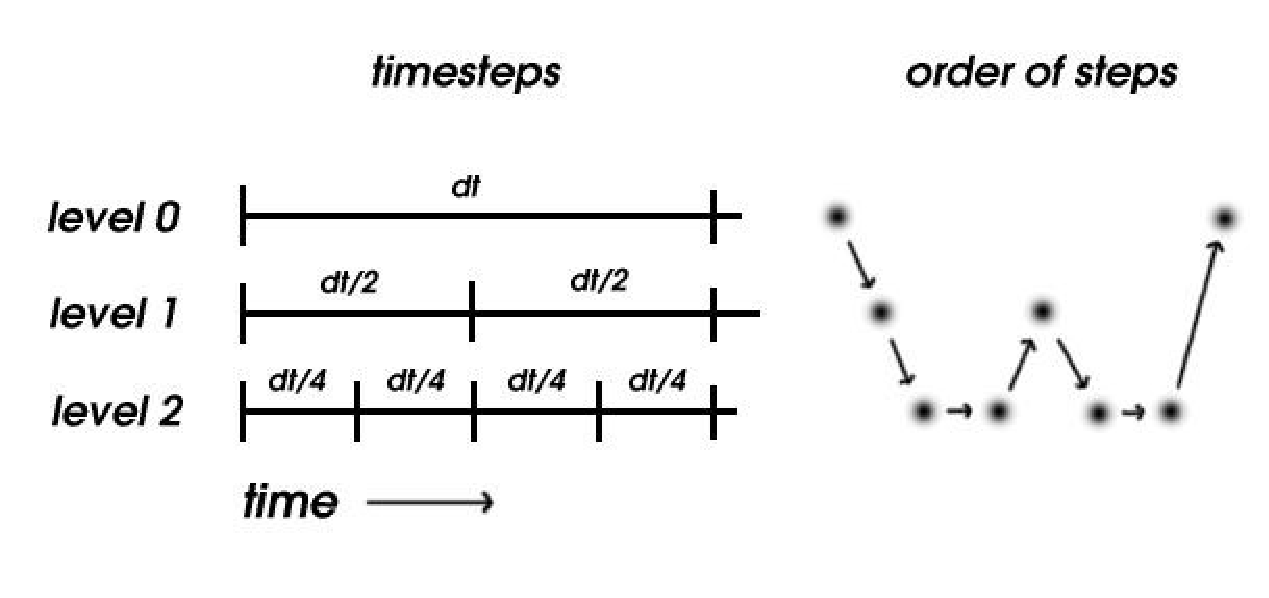
\includegraphics[width=0.6\textwidth]{figures/wcycle.eps}
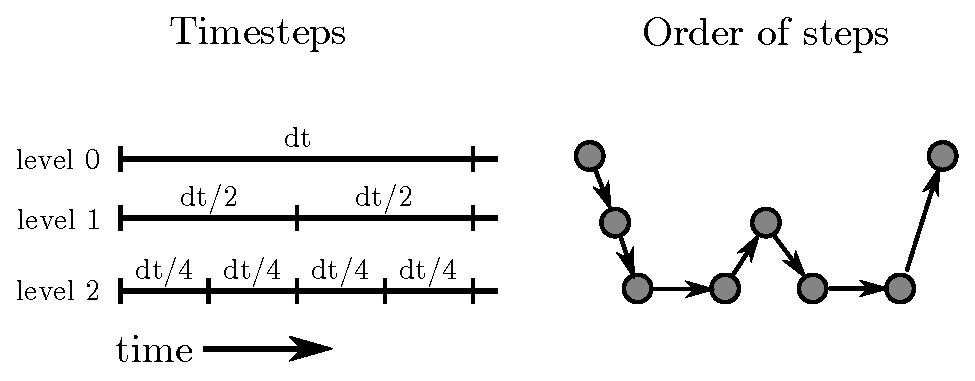
\includegraphics[width=0.6\textwidth]{figures/timestepping.eps}
\end{center}
\caption{\emph{Left:} Example of the timesteps on a 2-level AMR
  hierarchy.  \enzo\ does not restrict the timesteps on the finer levels
  to be a factor of $1/2^n$ smaller.  \emph{Right:} The order in which
  the AMR grids are evaluated on each level.\vspace{1ex}}
\label{fig:wcycle}
\end{figure}

Since interesting regions on the grid may move, the hierarchy must
adapt itself. This happens whenever a level has caught up to its
parent level, by entirely rebuilding the grids on that level and at
finer resolutions. Rebuilding is achieved by applying the grid
refinement criteria to the grids on that level and flagging zones that
require extra grids.  These criteria depend on the physical problem
being simulated; see Section~\ref{sec:refinement_criteria} for more
details.  Once a grid has a set of flagged cells, we apply a
machine-vision based algorithm \citep{Berger91} to find edges and
determine a good placement of subgrids.
%  These subgrids must not overlap one another, must cover all flagged
% cells and their neighbouring cells, and be above a preset efficiency
% threshold, where the efficiency of a cell is defined as the ratio of
% flagged cells to total cells. 
Once these new subgrids have been identified, the solution from the
next coarser grid is interpolated in order to initialize the values on
the new grids.  Finally, any overlap between new subgrids and old ones
is identified, and the prior solution within the regions of overlap is
copied to the new subgrids. This procedure is then repeated on the new
grids and in this way, the entire hierarchy (from the original level
examined and continuing on to all finer levels) is rebuilt.

\subsubsection{(Magneto)-hydrodynamic solver methods}

Four different (magneto)-hydrodynamic methods are implemented in
\enzo: (i) the hydrodynamic-only piecewise parabolic method (PPM)
developed by~\citet{1984JCoPh..54..174C} and extended to cosmology
by~\citet{1995CoPhC..89..149B}; (ii) the MUSCL-like Godunov scheme
\citep{1977JCoPh..23..276V} with or without magnetic fields and Dedner-based
divergence cleaning, described in more detail in
\citet{WangAbelZhang08} and \citet{WangAbel09}; (iii) a constrained
transport staggered MHD scheme \citep{Collins10}, and (iv) the
second-order finite difference hydrodynamics method described in
\zeus~\citep{Stone92a,Stone92b}.

\paragraph{Godunov PPM method (HD only)}

We begin with the direct-Eulerian PPM implementation.  This is an
explicit, higher-order accurate version of Godunov's method for ideal
gas dynamics with the spatially third-order accurate piecewise parabolic monotonic
interpolation and a nonlinear Riemann solver for shock capturing.  It
advances the hydrodynamic equations in the following steps:
%\begin{enumerate}
% \item 
(i) Construct monotonic parabolic interpolation of cell average data,
for each fluid quantity;
% \item 
(ii) Compute interface states by averaging the parabola over the
domain of dependence for each interface;
% \item 
(iii) Use interface data to solve the Riemann problem;
 %\item 
(iv) Difference the interface fluxes to update the cell average
quantities.
%\end{enumerate}

The PPM implementation does an excellent job of capturing strong
shocks across a few cells.  Multidimensional schemes are built up by
directional splitting and produce a method that is formally
second-order accurate in space and time and which explicitly conserves mass,
linear momentum, and energy \citep{Hawley84, Norman86}.  A variety of
Riemann solvers have been implemented.

As described in \citet{1995CoPhC..89..149B}, we modify the method for use in
hypersonic flows when the thermal energy $e$ is extremely small
compared to the total energy $E$.  This situation presents a problem
because in the total energy method the temperature is computed by
subtracting one large number from another (i.e. the kinetic energy
from the total energy), which tends to generate large numerical
inaccuracies. We overcome this difficulty by additionally solving a
thermal energy equation and using $e$ from this equation when we
expect the error to be large.

\paragraph{Godunov MUSCL (HD) with Dedner divergence cleaning (MHD)}
This solver was developed to attack problems in magnetic field
amplification during the formation of galaxies \citep{Wang:2009a} and
to understand the role of proto-stellar jets for the theory of star
formation \citep{Wang:2009b}. It combines the standard approach of
Godunov \citep{Godunov1959} for finite volume techniques with the
method of lines as described by \cite{leveque2002finite} and
\cite{toro-1997}. In addition, it implements the hyperbolic divergence
cleaning algorithm of \cite{2002JCoPh.175..645D}. It supports multiple
approximate Riemann solvers and non-ideal equations of
states. Consequently, this suite of solvers can be used for hydro and
magneto-hydrodynamic simulations. This class of solvers, as
well as a version of the PPM hydro solver, has been ported to
nVidia's CUDA framework, allowing \enzo\ to take advantage of modern
graphics hardware \citep{Wang:2010}.

\paragraph{Godunov MHD with Constrained Transport (MHD)}
This MHD method is second-order in time and space, and preserves the
divergence constraint, $\div \vecB = 0$, to machine precision
through the Constrained Transport (CT) method \citep{Collins10}.  CT, originally
described by \citet{Evans88}, updates the magnetic field with the curl
of an electric field, suitably formulated to preserve $\div
\vecB$.  We employ the CT methods described by \citet{Balsara99} and
\citet{Gardiner05} with the second-order hyperbolic
solver of \citet{Li08a} and the divergence free AMR scheme of
\citet{Balsara01}.

\paragraph{Second-order finite difference method (HD only)}

Lastly, we briefly describe the \zeus\ method, a finite difference
algorithm originally used in the \zeus\ code \citep{Stone92a}. Note
that \enzo\ is entirely independent of the \zeus\ code, and only the
hydrodynamical algorithm of \zeus\ has been implemented in \enzo; the
MHD and radiation-hydrodynamics schemes have not. The \zeus\ method
uses a staggered mesh such that velocities are face-centered, while
density and internal energy are cell-centered.  It splits the solution
up into two steps. The first is the so-called source step, in which
the momentum and energy values are updated to reflect the pressure and
gravity forces, including an artificial viscosity required for
stability. The second step, known as the transport step, accounts for
the advection of conserved quantities (mass, momentum, and energy)
across the grid.

\subsubsection{Gravity}

The current implementation of self-gravity in \enzo\ uses a Fast
Fourier Technique \citep{Hockney88} to solve Poisson's equation on the
root grid on each timestep.  The advantage of using this method is
that it is fast, accurate, and naturally allows both periodic and
isolated boundary conditions for the gravity, choices which are very
common in astrophysics and cosmology.  On subgrids, we interpolate the
boundary conditions from the parent grid (either the root grid or some
other subgrid). The Poisson equation is then solved on every timestep
using a multigrid technique on one subgrid at a time. Aside from
self-consistently calculating the gravitational potential arising from
the baryon fields and particles in the simulation, there are also a
number of options for specifying static gravitational fields, and in
fact including self-gravity is optional.

\subsubsection{N-body Dynamics}

Collisionless matter (e.g. dark matter, stars, etc.) is modeled with
particles that interact with the baryons only via gravity.  These
particles are advanced through a single timestep using a drift-kick-drift
algorithm \citep{Hockney88} to provide second-order accuracy even in
the presence of varying timesteps.  Since the particles follow the
collapse of structure, they are not adaptively refined.  Nor are there
duplicate sets of particles for each level; instead, each particle is
associated with the highest refined level available at its position in
the domain and particles are moved between grids as the hierarchy is
rebuilt. Thus a particle has the same timestep and feels the same
gravitational force as a grid at that refinement level.

Although the particles are fixed in mass once initialized (with the
exception of star particles, which can lose mass in the feedback
process), we can create them with any initial set of masses and
positions.  For example, in many cosmological simulations static
subgrids are included from the beginning in order to improve the
initial spatial and baryonic mass resolution, and these subgrid are
populated with lower mass particles to correspondingly improve the
collisionless mass resolution.
%% One particle per initial grid point seems to provide approximately
%% equal sampling between the dark matter and gas. \mqk{This
%% contradicts the conclusions of O'Shea et al. 2005 that an initial
%% grid twice as fine as the mean particle separation is necessary to
%% properly capture the abundance of low mass halos.}

\subsubsection{Chemistry}
\label{sec.ov.chem}

\enzo\ includes the capability of following up to 12 particle species
using a non-equilibrium chemical network.  The species can be turned
on in sets, with the simplest model including just atomic hydrogen and
helium (H, H$^+$, He, He$^+$, He$^{++}$, e$^-$), and more complete
models adding first species important for gas-phase molecular hydrogen
formation (H$^-$, H$_2$ and H$_2^+$), and then HD formation (HD, D,
D$^+$).
%(We note that a reduced version
%of the chemistry, used only with the flux-limited diffusion radiation
%transport, includes only hydrogen species.)
The cooling and heating due to these species is included (see the next
section). The solution of the rate equations is carried out using one
Jacobi iteration of an implicit Euler time discretization to ensure
stability. To ensure accuracy the rate equations are sub-cycled
within one hydrodynamic timestep, subject to the constraint that the
electron and neutral fractions do not change by more than 10\% in one
sub-cycle.

\subsubsection{Radiative Cooling and Heating}

\enzo\ can operate in a number of different modes with regard to
radiative cooling and heating. In the simplest mode, where the
multi-species flag is turned off and no individual chemical species
are tracked, the cooling rate is computed from a
simple temperature-dependent cooling function, taken from
\citet{SW87}.  If chemistry is turned on, then the code can include
cooling from all species of hydrogen and helium (including H$_2$) --
and the primordial cooling rates are computed in the same Jacobi iteration as the
chemistry.  It is also possible to include metal cooling based on a
set of multi-dimensional lookup tables computed with the
\textsc{Cloudy} code \citep{1998PASP..110..761F} as described in
\citet{2008MNRAS.385.1443S} and \citet{2011ApJ...731....6S}. Note that
the cooling and heating is most commonly treated in the optically-thin
limit, but the code can also follow radiative transfer in a limited
set of energy bins.

\subsubsection{Homogeneous radiation backgrounds}

The chemical networks and heating rates described in the previous
sections can be affected by external radiation fields, and the code
includes a number of pre-calculated meta-galactic UV radiation
backgrounds that are uniform in space but can vary in time.  These are
generally based on the redshift-dependent rates given in
\citet{1996ApJ...461...20H} and \citet{2012ApJ...746..125H}, but can
also include a uniform H$_2$ photo-dissociating background that is
either constant in time or varying as in \citet{WiseAbel05}.

\subsubsection{Radiation transport: ray tracing}

\enzo\ includes a photon-conserving radiative transfer algorithm that
is based on an adaptive ray-tracing method utilizing the HEALPix
pixelization of a sphere \citep{Abel02_RT}. Photons are integrated
outwards from sources using an adaptive timestepping scheme that
preserves accuracy in ionization fronts even in the optically-thin
limit. This has been coupled to the chemistry and cooling network to
provide ionization and heating rates on a cell-by-cell basis. The
method is described in detail (including numerous code tests) in
\citet{Wise11_Moray}.

\subsubsection{Radiation transport: Flux-limited diffusion}

A second option for radiative transfer is a moment-based method that
adds an additional field tracking the radiation energy density.  This
field is evolved using the flux-limited diffusion method, which
transitions smoothly between streaming (optically thin) and opaque
limits and is coupled to an ionization network of either purely
hydrogen, or both hydrogen and helium.  The
resulting set of linear equations is solved using the parallel HYPRE
framework.  Full details on the \enzo\ implementation of this method
can be found in \citet{ReynoldsHayesPaschosNorman2009}.

\subsubsection{Heat Conduction}

Heat conduction, both isotropic and anisotropic, can be included using
a sub-cycled, operator-split method.  The heat fluxes are computed
with simple second-order accurate finite differences, and stability is
ensured by restricting the timestep and using flux-limiters where
appropriate.

\subsubsection{Star Formation and Feedback}

A family of simple heuristic methods are used to model the formation
of stars and their feedback of metals and energy into the gas.  These
methods are based on the work of \citet{CO1992}, and involve the
identification of plausible sites of star formation based on a set of
criteria (for example, dense gas with a short cooling time, which is
both collapsing and unstable).  The local star formation rate is
computed using a range of methods, such as a density-dependent method
based on the Schmidt-Kennicutt relation \citep{K89}.  The affected gas
is converted into a star particle over a few dynamical times, and
metals and thermal energy are injected into the region surrounding the
star particle.  A related set of methods involves the simulation of
single Population III stars, rather than ensembles, and is calibrated
by \textit{ab initio} simulations of primordial star formation.

\subsubsection{Timestep constraints}

All grids on a given level are advanced with the same timestep.  This
time step is determined by first calculating the largest time step
allowed for each cell and for each physical process separately (except
for chemistry and heat conduction, which are sub-cycled).  The level
is then advanced with a timestep equal to the minimum over all of
these $\Delta t$.

%%% Local Variables:
%%% mode: latex
%%% TeX-master: "ms"
%%% End: 
